\section{Experimental Framework}
\label{sec:experiments}


To illustrate our theoretical results, we evaluate the predictive performance of the models as well as their ability  to capture homophily and preferential attachment on artificial and real networks.  

In the sequel of this section, we describe the evaluation measures and the datasets that we used for our experiments, before presenting the results.







\subsection{Measures for the Properties}

\textit{Homophily Indicators}

To evaluate homophily in a given attributed network, we use the measures introduced by \cite{largeron2015}, adapted from the test proposed by \cite{Easley2010}.  This test compares an expected homophily measure corresponding to the probability for two vertices to be similar with an observed homophily measure defined as the probability that two linked vertices are similar. More precisely, given a contingency table defined as follows:

$a = Card\{(i,j)\in V\times (V-1) / (i,j) \in E \land s(i,j)\}$\\
$b = Card\{(i,j)\in V\times (V-1) / (i,j) \in E \land \neg{s(i,j)}\}$\\ 
$c = Card\{(i,j)\in V\times (V-1) / (i,j) \notin E \land s(i,j)\}$\\
$d = Card\{(i,j)\in V\times (V-1) / (i,j) \notin E \land \neg{s(i,j)}\}$\\
%$\frac{N*(N-1)}{2}$ is the total count of  the cells in the contingency table.\\

where  s(i,j) indicates that i and j are considered as similar, observed homophily, denoted $H_{obs}$, is given by $\frac{a}{a+b}$.\\
This measure  is equal to 1 when all the pairs of linked vertices are similar. Consequently, high values suggest an homophily effect.

Moreover, $H_{obs}$ can be compared with an expected measure, $H_{expec}$, defined by  $ \frac{a+c}{a+b+c+d}$.\\

If the expected measure is significantly less than the observed measure, then there is evidence for homophily.\\

\textit{Preferential attachment}

Preferential attachment leads to networks characterized by a degree distribution with heavy tail which can take the form of a power law. To evaluate this property, we  plot the degree distributions in log log scale for the original network and the generated network. Comparaison of the degree distribution with a straight line gives us a qualitative measure for the preferential attachment.\\

\textit{Preditive performance}

The predictive performance of models is evaluated according \textbf{Adrien ?}.\\

\subsection{Datasets}
In our experiments, we consider four artificial networks and two real networks.\\

\textit{Artificial networks}

The artificial networks have been generated with ANC-Generator \cite{largeron2015}. This generator has been chosen because it allows to build attributed graphs with community structure faithfully following the known properties of real-world networks such as preferential attachment and homophily. 
Moreover, by modifying the parameters, these properties can be weakened. Finally, ANC-Generator is available under the terms of the GNU Public Licence and the parameters can be shared for experiments reproducibility. 

Four artificial networks have been generated, each one corresponding to a configuration  regarding the properties of interest.
Table \ref{table:artificial_networks} summarizes these four configurations while Table \ref{table:generatorparameter} gives the parameter setting used to built these artificial networks. Both properties are verified in the first network ($Network1 b/h$) whereas none of them is checked in the $Network3 -b/-h$.  There is only an evidence for homophily in the network $Network4 -b/h$ and  preferential attachment in the network  $Network2 b/-h$.\\ 

\begin{table} \label{table:artificial_networks}
    \caption{Artificial networks properties.}
\begin{tabular}{lrrrr}
\hline                                                                             
 Networks   &  Preferential attachment    &  Homophily    \\                 
\hline                                                                             
$Network1~b/h$ & yes&yes  \\
$Network2~b/-h$  & yes&no   \\
$Network3~-b/-h$ &no &no   \\
$Network4~-b/h$ &no &yes  \\
\hline                                                                             
\end{tabular}  
\end{table}


\begin{table} \label{table:generatorparameter}
    \caption{Parameter setting.}
\begin{tabular}{lrrrr}
\hline                                                                             
 Networks   &  Parameters and seed used to generate the network in Dancer    \\                 
\hline                                                                             
$Network1~b/h$ &    \\
$Network2~b/-h$  &  \\
$Network3~-b/-h$ &   \\
$Network4~-b/h$ &  \\
\hline                                                                             
\end{tabular}  
\end{table}

 \textbf{retrouver parametrage}
 \textbf{ajouter commentaire sur properties}

% \textit{Real networks}
\textit{Real networks}

We evaluate also the models on two  real networks.
The first one \footnote{available at:} is built from an online community of 1899 students from the University of California. Each node corresponds to a user and a directed edge represents a sent message. 
The second one \footnote{available at:} is an internal email communication network between employees of a mid-sized manufacturing company. Each vertex is associated to an employee and an oriented link represents like previously a sent email.

Table 1 summarizes basic characteristics of these synthetic and real datasets \textbf{ Mettre nombre de sommets, de liens}.


\begin{figure}[h]
	\centering
	
	\minipage{0.25\textwidth}
	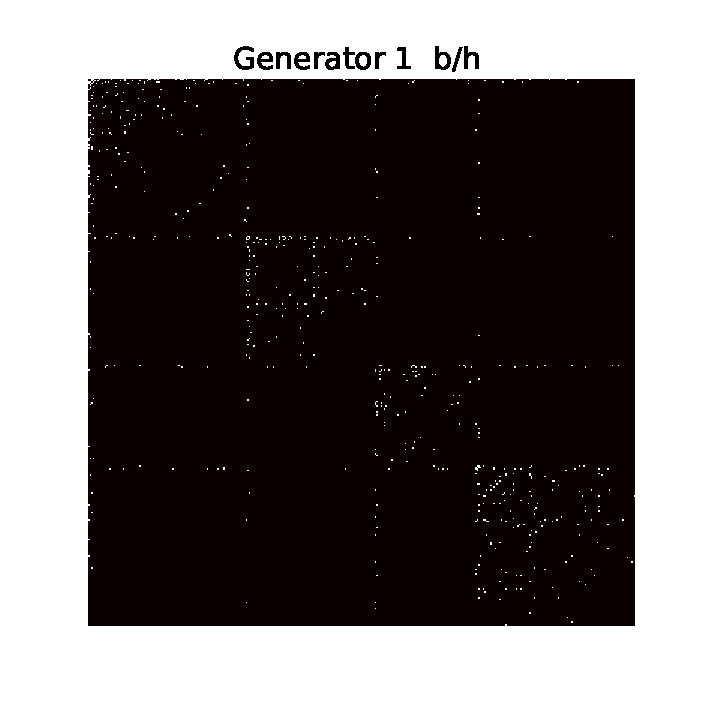
\includegraphics[scale=0.4]{img/g1}
	\endminipage
	\minipage{0.25\textwidth}
	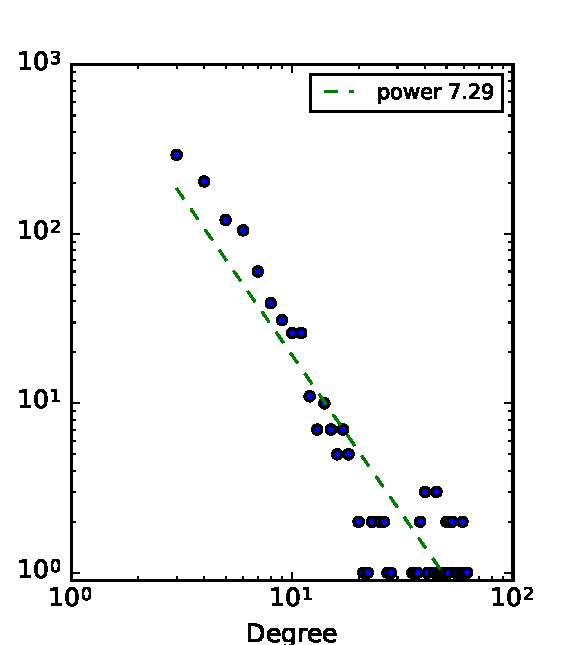
\includegraphics[scale=0.4]{img/g1_d}
	\endminipage
	\vspace{-0.4cm}
	\minipage{0.25\textwidth}
	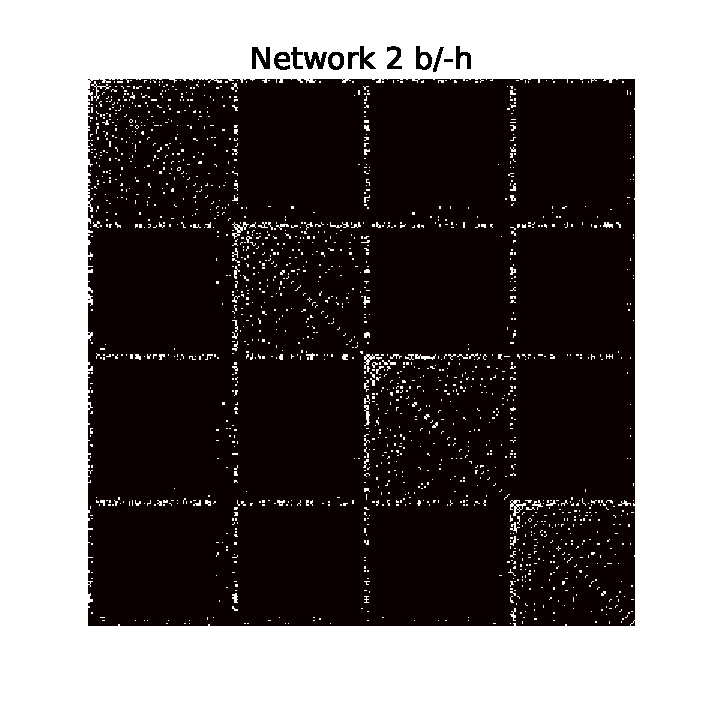
\includegraphics[scale=0.4]{img/g2}
	\endminipage
	\minipage{0.25\textwidth}
	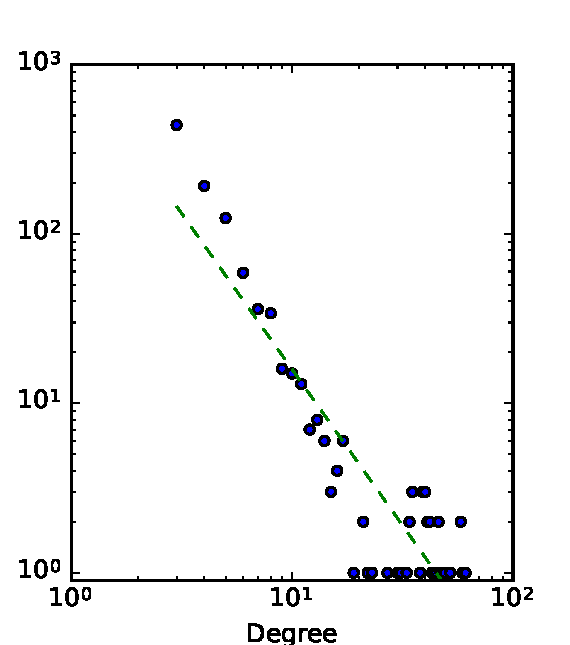
\includegraphics[scale=0.4]{img/g2_d}
	\endminipage
	\vspace{-0.4cm}
	\minipage{0.25\textwidth}
	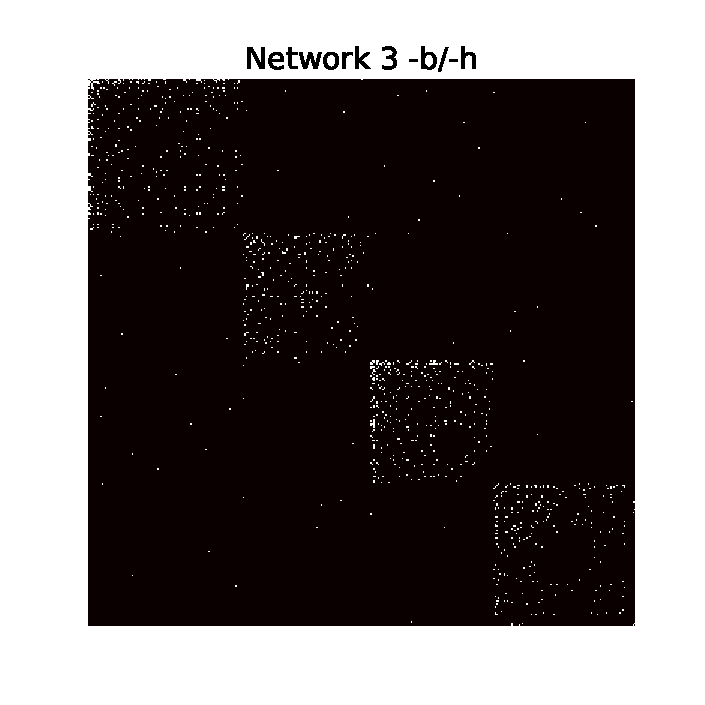
\includegraphics[scale=0.4]{img/g3}
	\endminipage
	\minipage{0.25\textwidth}
	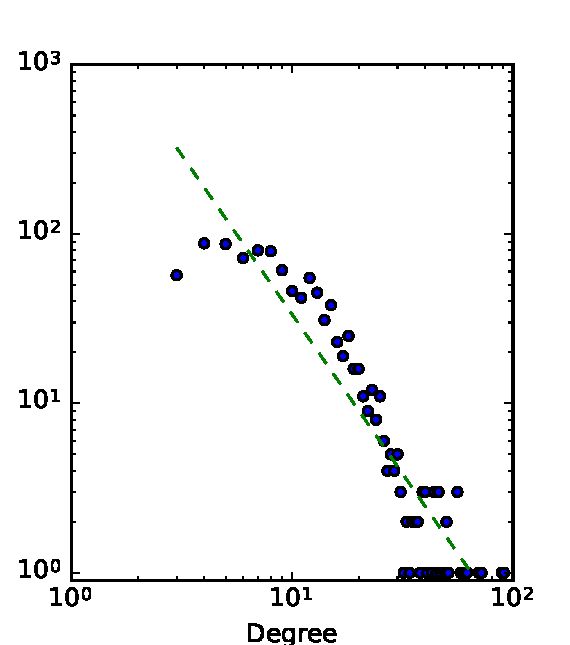
\includegraphics[scale=0.4]{img/g3_d}
	\endminipage
	\vspace{-0.4cm}
	\minipage{0.25\textwidth}
	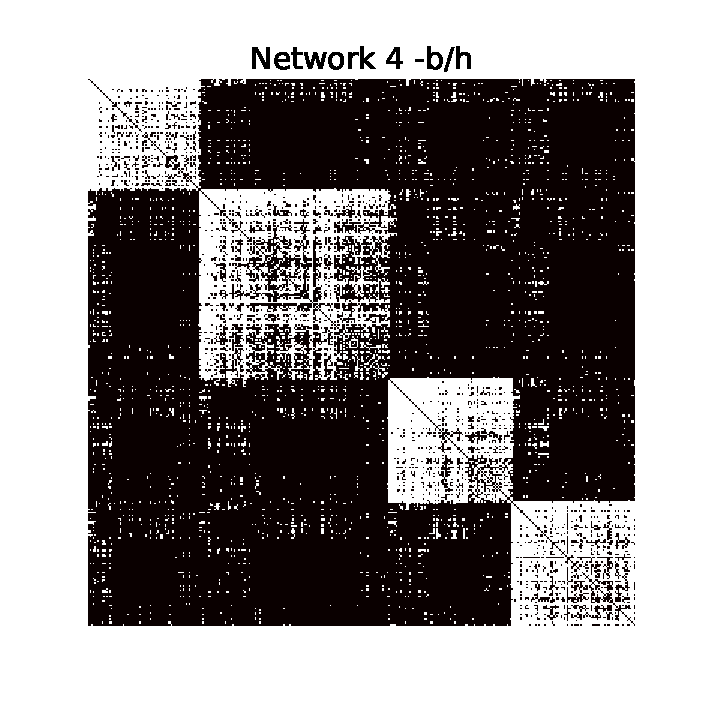
\includegraphics[scale=0.4]{img/g4}
	\endminipage
	\minipage{0.25\textwidth}
	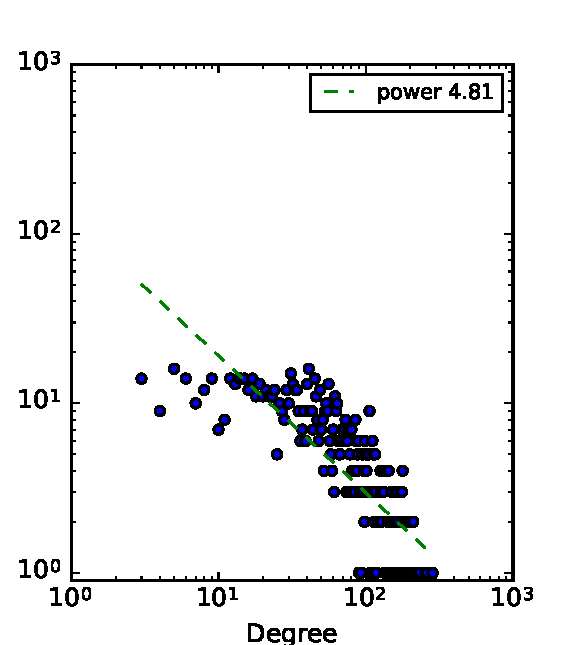
\includegraphics[scale=0.4]{img/g4_d}
	\endminipage
	
	\caption{Synthetic Networks. (left) adjacency matrix. (right) degree distribution}
	\label{fig:synt_graph}
\end{figure}



\begin{figure}[h]
	\centering
	

	\minipage{0.25\textwidth}
	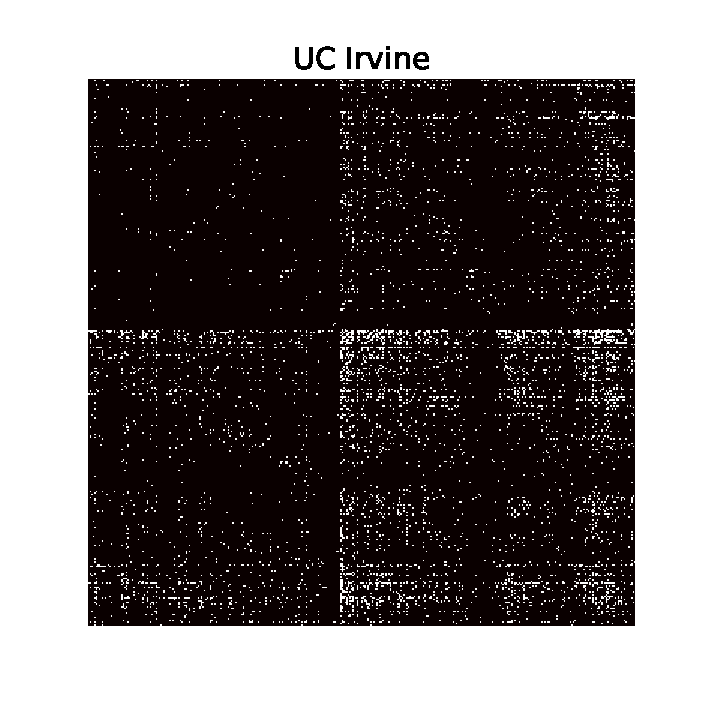
\includegraphics[scale=0.4]{img/irvine}
	\endminipage
	\minipage{0.25\textwidth}
	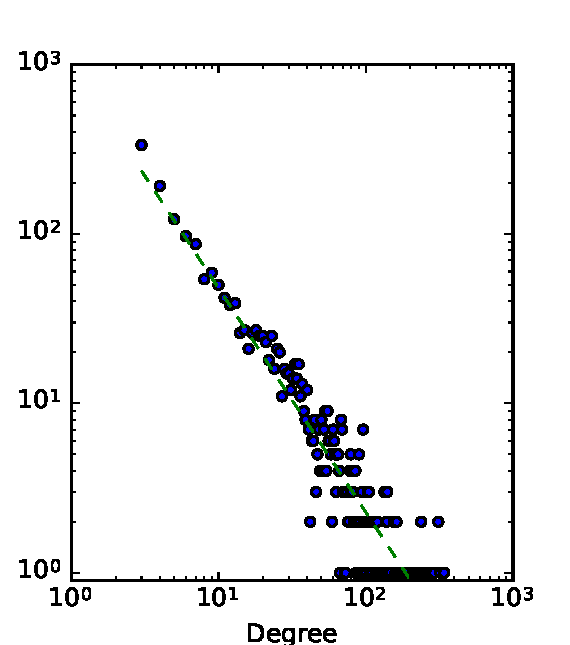
\includegraphics[scale=0.4]{img/irvine_d}
	\endminipage
		\vspace{-0.4cm}
	\minipage{0.25\textwidth}
	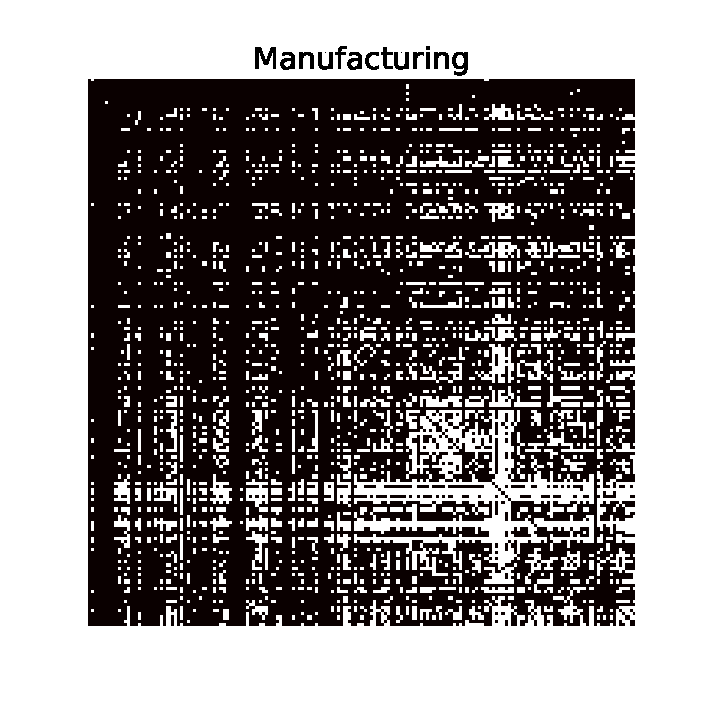
\includegraphics[scale=0.4]{img/manufacturing}
	\endminipage
	\minipage{0.25\textwidth}
	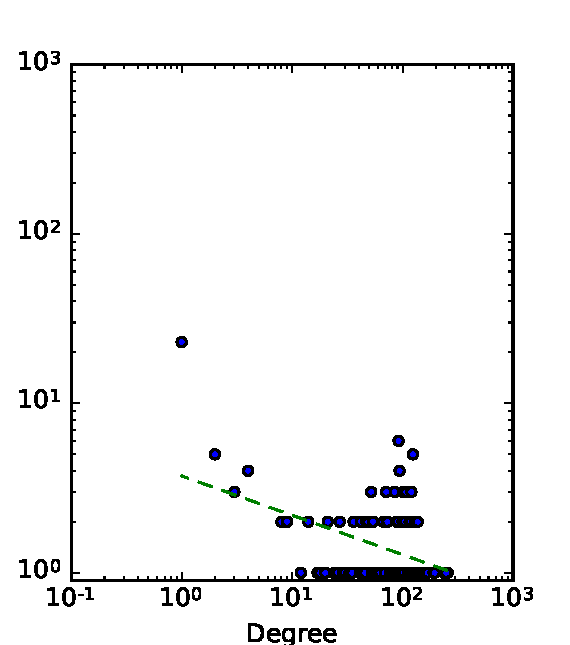
\includegraphics[scale=0.4]{img/manufacturing_d}
	\endminipage
	\caption{Real Networks. (left) adjacency matrix. (right) degree distribution}
	\label{fig:real_graph}
\end{figure}



\subsection{Evaluation Protocol}
For each datasets described,  we run a MCMC inference consisting of 200 iterations to learn the posterior distribution of each the IMMSB model and ILFM, described in \ref{sec:models}. For IMMSB, concentration parameters of HDP were optimized following \cite{HDP} using vague gamma priors $\alpha_0 \sim \text{Gamma}(1,1)$ and $\gamma \sim \text{Gamma}(1,1)$. The parameter for the matrix weights were fixed to $\lambda_0=\lambda_1=0.1$. For ILFM, the IBP hyper-parameter was fixed to $\alpha=0.5$ and the weights hyper-parameter to $\sigma_w = 1$.

Our evaluation rely then in two strategy:


\subsubsection{Predictive performance}
We evaluate the performance prediction of the models by building a training set and a testing set from the original datasets. Because the burstiness has a strong impact os the sparsity of the underlying graph, we face a very unbanlanced challenge. Considering this fact, we used two different strategy for building our testing set, in order to assess the impact of the sparsity:

\paragraph{Unbalanced testing set}
We separate our datasets into a training set representing 80 \% of the size of the network, and 20\% for a testing set, randomly chosen. As the dataset has a small density of edges, this testing set ends up with very small amout of edges.

\paragraph{Balanced testing set}
In order to create a balanced testing set, we pick randomly 20 \% of the edges of the network and the same amount of non-links. The testing ends up balanced but it represents a small proportion of the dataset.~\\


We performed a predictive analysis on the testing set and compared the predictive performance of each models with regards to the properties of the network. 
The predictive performance of models is calculated using a traditional precision and recall measures for the predicted links, that we calculated as follows:\\
\begin{align}
    \mathrm{precision}_{V} = Equation precision to complete... \\
    \mathrm{recall}_{V} = Equation recall to complete...
\end{align}


The table \ref{table:unbalanced} and table \ref{table:balanced} respectively shows the overall precision, edge precision and recall results respectively for unbalanced case and tha balance case. Additionnally, the tables show results for several initialization for the number of features $K$ for both models. The last colulmn show the number of latent features to which latent models have converged.

\subsubsection{Generative network}
We consider the generative ability of the models to build new \emph{synthetic} networks based on the information learned on the data. This can be expressed by the predictive likelihood given only the hyperparameters $h$ and the training data:
\begin{equation}
    \pr(Y_{new} |Y, h) = \int_{\M} \pr(Y_{new} |Y,\M, h)\pr(\M |, h)d\M
\end{equation}

The generative graph is the expectation of the predective likelihood on the model. The expectation of the generative graph is then given by the bilinear form, according to \ref{MFDCA}:
\begin{equation}
    \E_\M[Y_{new} | Y, \M] = \sigma(F \Phi F^T)
\end{equation}


The figure \ref{fig:gen_graph} shows the mean and variance of the degrees distribution of graphs generated by the ILFRM and the IMMSB when fitted on the synthetic dataset \ref{sec:datasets}.


\subsection{Results}

\subsubsection{Unbanlanced data}

\paragraph{Results for IMMSB}

For all predictive measure, the overall precision, precision for edge and the recall for edge are better for bursty networks, exept for the Network 4. This is because the density of the latter is higher than the other who make the prediction on this network less inbanlance than the other

On bursty networks, it appears that IMMSB has a tendancy to perform better on the networks where homophily is not strongly present. This can be explain by the fact that IMMSB allows relation between classes, and because strong homophily is correlated to more dense community in the synthetic network.


This observation confirm that IMMSB can capture burstiness and slighly better on slighly homophilic network.

\paragraph{Results for ILFM}
Resulst for ILFM show that the models converged to a hihger number of features for networks that are bursty. Even though the number of feature is smaller for the less bursty network, ILFM achive better  results on edge precision an recall.

\subsubsection{Comparison of models}
In most case, ILFM performs better than IMMSB but the difference is less significative on bursty networks.

\subsubsection{Balanced data}
\paragraph{Results for IMMSB}

\paragraph{Results for ILFM}
ILFM confirm his tendancy to learn more features on bursty networks. Nevertheless the overall precision and the recall remains significantly better whithin the non-bursty networks. Moreover the overall precision and the recall is significantly better for the strongly homophilic networks.

\paragraph{Comparison of models}

\begin{table} \label{table:real1}
    \caption{IMMSB prediction performance results on real networks, for several feature size initialization.}
\begin{tabular}{lrrrr}
\hline                                                                             
 immsb / mask all   &        5 &       10 &       15 &       20 \\                 
\hline                                                                             
fb\_uc & & & & \\
manufacturing  & & & & \\
\hline                                                                             
\end{tabular}  
\end{table}

 

\begin{table} \label{table:real2}
    \caption{ILFM predictive performance result on real networks}
\begin{tabular}{lrrrr}
\hline
 ILFRM / mask all   &     global &   precision &      recall &   K-\ensuremath{>} \\
\hline
fb\_uc& & & & \\
manufacturing  & & & & \\
\hline
\end{tabular}  
\end{table}

Our results confirm the theoretical analysis on nonparametric models, concerning their affinity to the preferential attachment effect and the homophily effect.

%Our experiments evaluate the preferential attachment and the local preferential attachment on the learned communities trough respectively the distribution of degrees in the networks and inside the communities.


\begin{figure}[h]
	\centering
	
	\minipage{0.25\textwidth}
	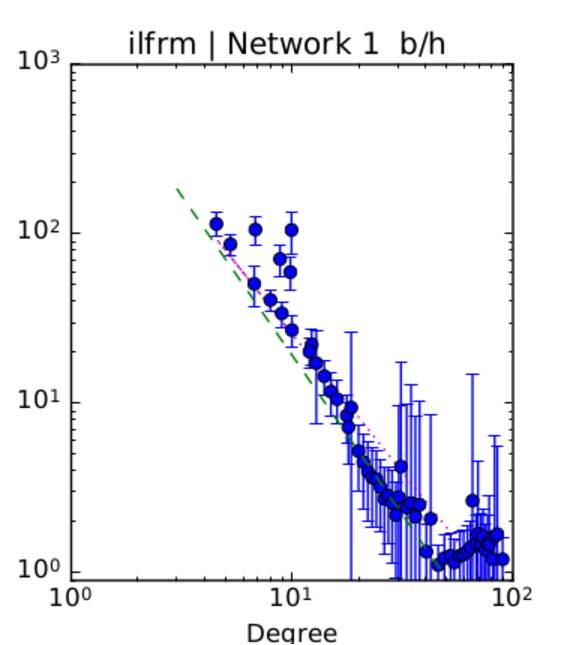
\includegraphics[scale=0.4]{img/ilfrm_g1_d}
	\endminipage
	\minipage{0.25\textwidth}
	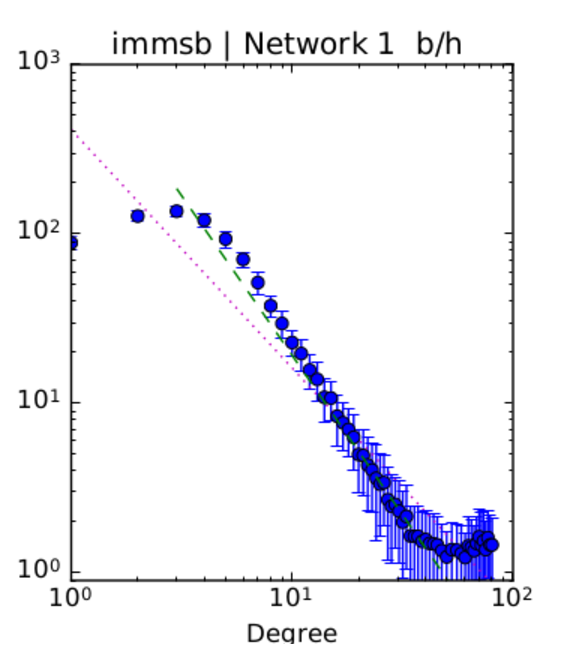
\includegraphics[scale=0.4]{img/immsb_g1_d}
	\endminipage
	\vspace{-0.4cm}
	\minipage{0.25\textwidth}
	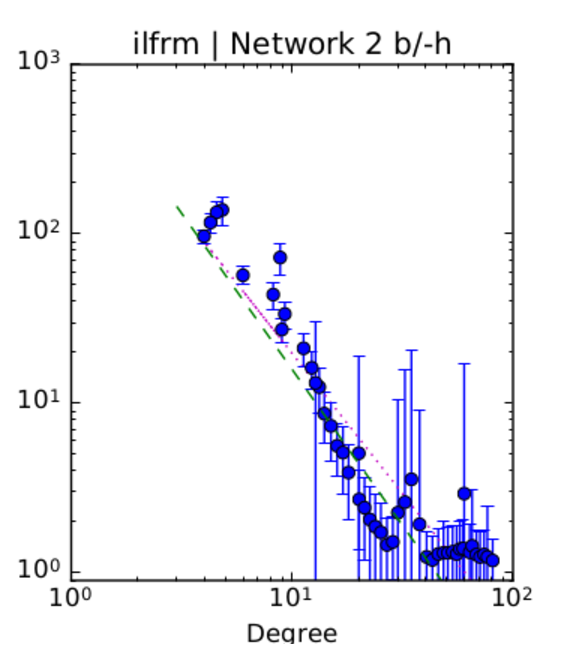
\includegraphics[scale=0.4]{img/ilfrm_g2_d}
	\endminipage
	\minipage{0.25\textwidth}
	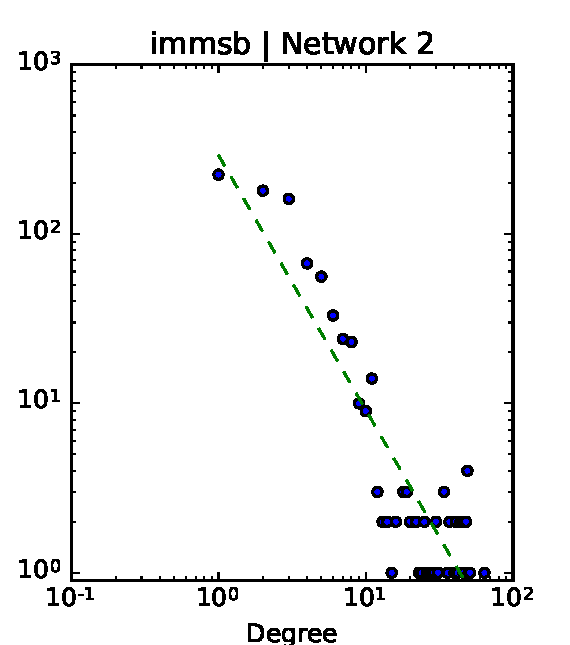
\includegraphics[scale=0.4]{img/immsb_g2_d}
	\endminipage
	\vspace{-0.4cm}
	\minipage{0.25\textwidth}
	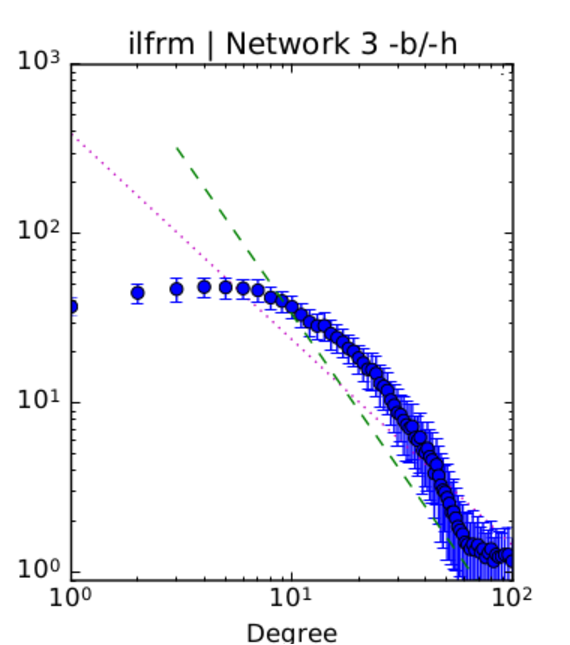
\includegraphics[scale=0.4]{img/ilfrm_g3_d}
	\endminipage
	\minipage{0.25\textwidth}
	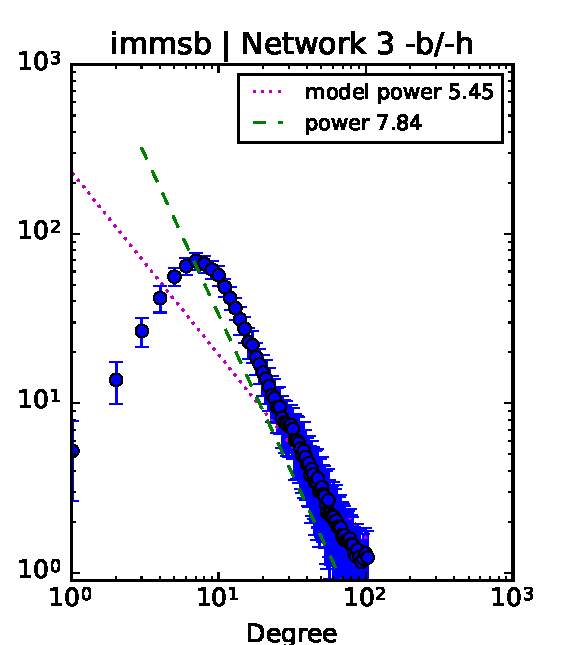
\includegraphics[scale=0.4]{img/immsb_g3_d}
	\endminipage
	\vspace{-0.4cm}
	\minipage{0.25\textwidth}
	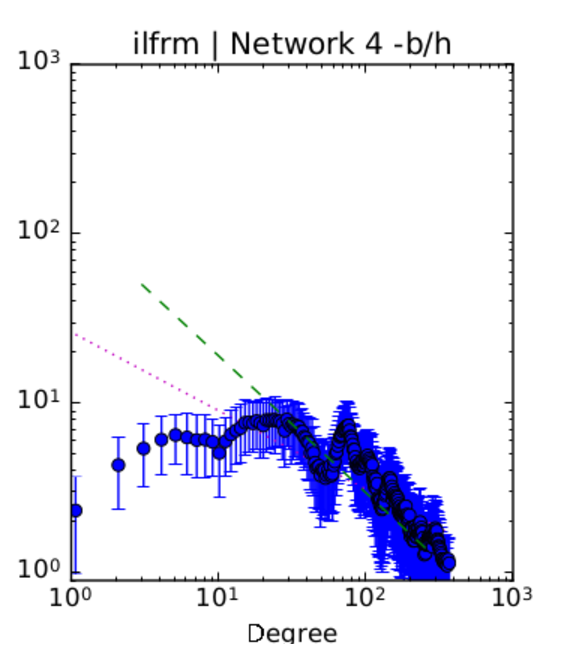
\includegraphics[scale=0.4]{img/ilfrm_g4_d}
	\endminipage
	\minipage{0.25\textwidth}
	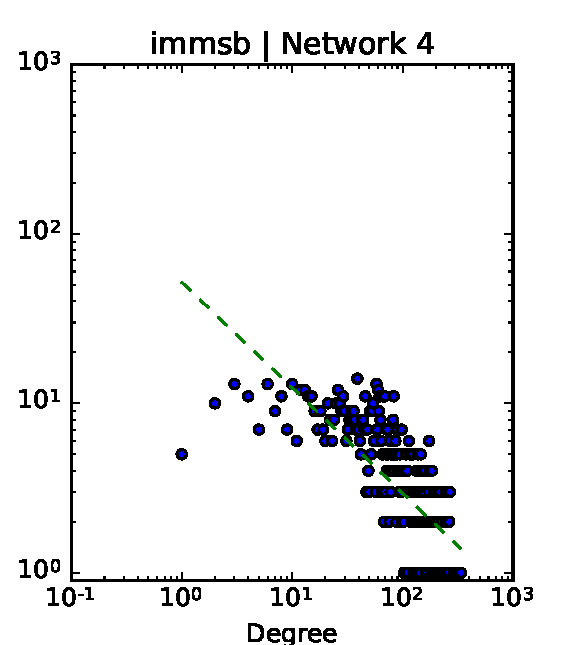
\includegraphics[scale=0.4]{img/immsb_g4_d}
	\endminipage
	
	\caption{Generated Networks with Latent Models}
	\label{fig:gen_graph}
\end{figure}



% Debug 12 / MASK all

% K = 5

\begin{table*}[h] \label{table:unbalanced}
\caption{Predictive Performance on a UnBalanced Testing set}
	\begin{minipage}[h]{0.45\linewidth} 
K = 5\hspace{5pt}
\begin{tabular}{lllll}
\hline
 IMMSB   &   global &   precision &   recall &    K-\ensuremath{>} \\
\hline
 Network1 b/h         &    0.990 &       0.029 &    0.032 & 5.0 $\pm$ 0.0 \\
 Network2 b/-h       &    0.992 &       0.032 &    0.034 & 5.0 $\pm$ 0.0 \\
 Network3 -b/h       &    0.979 &       0.031 &    0.034 & 5.0 $\pm$ 0.0 \\
 Network4 -b/-h       &    0.887 &       0.151 &    0.192 & 5.0 $\pm$ 0.0 \\

\hline
\end{tabular}
\end{minipage}
\hspace{0.8cm}
\begin{minipage}[h]{0.45\linewidth}
\begin{tabular}{lllll}
\hline
  ILFRM & global &   precision &   recall &     K-\ensuremath{>} \\
\hline
 Network1 b/h       &    0.990 &       0.051 &    0.053 & 13.4 $\pm$ 0.8    \\
 Network2 b/-h     &    0.992 &       0.044 &    0.045 & 14.0 $\pm$ 2.0    \\
 Network3 -b/h     &    0.982 &       0.114 &    0.116 & 10.0 $\pm$ 2.1 \\
 Network4 -b/-h     &    0.926 &       0.389 &    0.393 & 7.2 $\pm$ 1.6     \\

\hline
\end{tabular}
\end{minipage}

% K = 10

	\begin{minipage}[h]{0.45\linewidth} 
K = 10
\begin{tabular}{lllll}
Network1 b/h         &    0.990 &       0.044 &    0.046 & 10.0 $\pm$ 0.0 \\
 Network2 b/-h       &    0.992 &       0.039 &    0.045 & 10.0 $\pm$ 0.0 \\
 Network3 -b/h       &    0.979 &       0.030 &    0.035 & 10.0 $\pm$ 0.0 \\
 Network4 -b/-h       &    0.897 &       0.202 &    0.238 & 10.0 $\pm$ 0.0 \\

\hline
\end{tabular}
\end{minipage}
\hspace{0.8cm}
\begin{minipage}[h]{0.45\linewidth}
\begin{tabular}{lllll}
 Network1 b/h       &    0.990 &       0.049 &    0.053 & 17.2 $\pm$ 2.8 \\
 Network2 b/-h     &    0.992 &       0.047 &    0.051 & 17.2 $\pm$ 2.1 \\
 Network3 -b/h     &    0.982 &       0.132 &    0.132 & 12.2 $\pm$ 2.0 \\
 Network4 -b/-h     &    0.934 &       0.448 &    0.447 & 9.2 $\pm$ 1.2 \\

\hline
\end{tabular}
\end{minipage}

% K = 15

	\begin{minipage}[h]{0.45\linewidth} 
K = 15
\begin{tabular}{lrrrr}
 Network1 b/h         &    0.990 &       0.038 &    0.041 & 15.0 $\pm$ 0.0 \\
 Network2 b/-h       &    0.992 &       0.036 &    0.038 & 15.0 $\pm$ 0.0 \\
 Network3 -b/h       &    0.979 &       0.029 &    0.032 & 15.0 $\pm$ 0.0 \\
 Network4 -b/-h       &    0.898 &       0.207 &    0.245 & 15.0 $\pm$ 0.0 \\

\hline
\end{tabular}
\end{minipage}
\hspace{0.8cm}
\begin{minipage}[h]{0.45\linewidth}
\begin{tabular}{lrrrr}
 Network1 b/h       &    0.990 &       0.050 &    0.053 & 20.6 $\pm$ 2.1 \\
 Network2 b/-h     &    0.992 &       0.049 &    0.055 & 21.2 $\pm$ 2.1 \\
 Network3 -b/h     &    0.983 &       0.164 &    0.166 & 17.2 $\pm$ 1.3 \\
 Network4 -b/-h     &    0.939 &       0.499 &    0.501 & 14.8 $\pm$ 0.4    \\

\hline
\end{tabular}
\end{minipage}

% K = 20

	\begin{minipage}[h]{0.45\linewidth} 
K = 20
\begin{tabular}{lrrrr}

 Network1 b/h          &   0.9899 &      0.0348 &   0.0375 & 20 \\
 Network2 b/-h       &   0.9923 &      0.0494 &   0.0590 & 20 \\
 Network3 -b/-h      &   0.9794 &      0.0289 &   0.0338 & 20 \\
 Network4 -b/h        &   0.9067 &      0.2646 &   0.3034 & 20 \\
\hline
\end{tabular}
\end{minipage}
\hspace{0.8cm}
\begin{minipage}[h]{0.45\linewidth}
\begin{tabular}{lrrrr}
Network1 b/h       &   0.9902 &      0.0641 &   0.0626 &  23 \\
Network2 b/-h     &   0.9915 &      0.0477 &   0.0636 & 17 \\
Network3 -b/h     &   0.9827 &      0.1523 &   0.1518 &  20 \\
Network4 -b/-h     &   0.9396 &      0.4986 &   0.5053 &  22 \\
\hline
\end{tabular}
\end{minipage}
\end{table*}


%%%%%%%%%%%%%%%%%%%%%%%%%%%%%%%%%%%%%%%%%%%%%%%%%%%%%%%%%%%%%%%%%%%%
%%%%%%%%%%%%%%%%%%%%%%%%%%%%%%%%%%%%%%%%%%%%%%%%%%%%%%%%%%%%%%%%%%%%
%%%%%%%%%%%%%%%%%%%%%%%%%%%%%%%%%%%%%%%%%%%%%%%%%%%%%%%%%%%%%%%%%%%%
%%%%%%%%%%%%%%%%%%%%%%%%%%%%%%%%%%%%%%%%%%%%%%%%%%%%%%%%%%%%%%%%%%%%
%%%%%%%%%%%%%%%%%%%%%%%%%%%%%%%%%%%%%%%%%%%%%%%%%%%%%%%%%%%%%%%%%%%%
%%%%%%%%%%%%%%%%%%%%%%%%%%%%%%%%%%%%%%%%%%%%%%%%%%%%%%%%%%%%%%%%%%%%


% Debug 11 / MASK 1

% K = 5

\begin{table*}[h] \label{table:balanced}
\caption{Predictive Performance on a Balanced Testing set}
	\begin{minipage}[h]{0.45\linewidth} 
K =  5\hspace{5pt}
\begin{tabular}{lrlll}
\hline
 IMMSB   &   global &   precision &   recall &    K-\ensuremath{>} \\
\hline
 Network1 b/h          &    0.549 &       0.758 &    0.022 & 5.0 $\pm$ 0.0 \\
 Network2 b/-h        &    0.558 &       0.834 &    0.019 & 5.0 $\pm$ 0.0 \\
 Network3 -b/h        &    0.527 &       0.729 &    0.027 & 5.0 $\pm$ 0.0 \\
 Network4 -b/-h        &    0.557 &       0.743 &    0.162 & 5.0 $\pm$ 0.0 \\

\hline
\end{tabular}
\end{minipage}
\hspace{0.8cm}
\begin{minipage}[h]{0.45\linewidth}
\begin{tabular}{lrlll}
\hline
 ILFRM   &   global &   precision &   recall &     K-\ensuremath{>} \\
\hline
 Network1 b/h        &    0.568 &       0.912 &    0.047 & 13.6 $\pm$ 2.3 \\
 Network2 b/-h      &    0.574 &       0.893 &    0.041 & 16.4 $\pm$ 3.4 \\
 Network3 -b/h      &    0.571 &       0.912 &    0.100 & 9.2 $\pm$ 1.3 \\
 Network4 -b/-h      &    0.668 &       0.906 &    0.362 & 7.6 $\pm$ 1.3 \\

\hline
\end{tabular}
\end{minipage}

% K = 10

	\begin{minipage}[h]{0.45\linewidth} 
K = 10
\begin{tabular}{lrrrr}
 Network1 b/h          &    0.558 &       0.842 &    0.028 & 10.0 $\pm$ 0.0 \\
 Network2 b/-h        &    0.567 &       0.926 &    0.034 & 10.0 $\pm$ 0.0 \\
 Network3 -b/h        &    0.530 &       0.776 &    0.027 & 10.0 $\pm$ 0.0 \\
 Network4 -b/-h        &    0.567 &       0.764 &    0.184 & 10.0 $\pm$ 0.0 \\

\hline
\end{tabular}
\end{minipage}
\hspace{0.8cm}
\begin{minipage}[h]{0.45\linewidth}
\begin{tabular}{lrrrr}
 Network1 b/h        &    0.556 &       0.928 &    0.044 & 17.2 $\pm$ 2.0 \\
 Network2 b/-h      &    0.573 &       0.935 &    0.041 & 17.6 $\pm$ 3.2    \\
 Network3 -b/h      &    0.579 &       0.947 &    0.118 & 12.8 $\pm$ 0.9 \\
 Network4 -b/-h      &    0.718 &       0.943 &    0.457 & 10.8 $\pm$ 0.7 \\

\hline
\end{tabular}
\end{minipage}

% K = 15

	\begin{minipage}[h]{0.45\linewidth} 
K = 15
\begin{tabular}{lrrrr}
 Network1 b/h          &    0.555 &       0.871 &    0.035 & 15.0 $\pm$ 0.0 \\
 Network2 b/-h        &    0.570 &       0.854 &    0.030 & 15.0 $\pm$ 0.0 \\
 Network3 -b/h        &    0.532 &       0.728 &    0.027 & 15.0 $\pm$ 0.0 \\
 Network4 -b/-h        &    0.565 &       0.757 &    0.178 & 15.0 $\pm$ 0.0 \\

\hline
\end{tabular}
\end{minipage}
\hspace{0.8cm}
\begin{minipage}[h]{0.45\linewidth}
\begin{tabular}{lrrrr}
 Network1 b/h        &    0.569 &       0.928 &    0.046 & 20.8 $\pm$ 1.3 \\
 Network2 b/-h      &    0.564 &       0.903 &    0.042 & 21.6 $\pm$ 2.4 \\
 Network3 -b/h      &    0.594 &       0.952 &    0.153 & 18.0 $\pm$ 0.8 \\
 Network4 -b/-h      &    0.723 &       0.945 &    0.467 & 15.0 $\pm$ 0.0    \\

\hline
\end{tabular}
\end{minipage}

% K = 20

	\begin{minipage}[h]{0.45\linewidth} 
K = 20
\begin{tabular}{lrrrr}

 Network1 b/h           &   0.5501 &      0.8980 &   0.0425 & 20 \\
 Network2 b/-h        &   0.5734 &      0.9615 &   0.0326 & 20 \\
 Network3 -b/-h       &   0.5286 &      0.6456 &   0.0255 & 20 \\
 Network4 -b/h         &   0.5577 &      0.7475 &   0.1662 & 20 \\
\hline
\end{tabular}
\end{minipage}
\hspace{0.8cm}
\begin{minipage}[h]{0.45\linewidth}
\begin{tabular}{lrrrr}
 Network1 b/h         &   0.5428 &      0.9737 &   0.0359 &  21 \\
 Network2 b/-h      &   0.5577 &      0.8462 &   0.0389 &  20 \\
 Network3 -b/-h     &   0.5997 &      0.9503 &   0.1630 &  22 \\
 Network4 -b/-h      &   0.7291 &      0.9473 &   0.4813 & 20 \\
\hline
\end{tabular}
\end{minipage}
\end{table*}



